\subsection{Ensayo sin Carga}

Como primer ensayo, se realizaron mediciones de la tensión en el bobinado primario $V_p$, junto con las tensiones del punto medio de cada pata del puente de transistores, $V_p^+$ y $V_p^-$. Todas estas pruebas se realizaron con distintos niveles de desfase entre las señales de las patas del puente, que son equivalentes a distintos valores de ciclo de trabajo del secundario $D_{sec}$.\\

Los terminales de entrada correspondientes a la pila de combustible fueron conectados a la fuente de laboratorio HP6010A, entregando una tensión continua de \SI{30}{\volt}. Sin embargo, como esta fue la primer prueba realizada sobre el convertidor CC-CC, se llevó a cabo sin ningún tipo de carga, dejando los terminales correspondientes a ambos bobinados del transformador a circuito abierto. De esta manera, no existe circulación de corriente, y no se corre el riesgo de destruir algún componente en caso de una falla inesperada del circuito, como podría ser un cortocircuito.\\

El objetivo de este ensayo es relevar el correcto funcionamiento de los circuitos de excitación del puente, compuestos por los dos drivers 2ED21834-S06J. Se debe verificar que sean capaces de disparar los IRFP150, y que funcionen correctamente los circuitos de bootstrap necesarios para activar los transistores del lado alto.\\

\subsubsection{Resultados}

\begin{figure}[h]
    \centering
    \hspace{0.5em}
    \begin{subfigure}{0.47\textwidth}
        \centering
        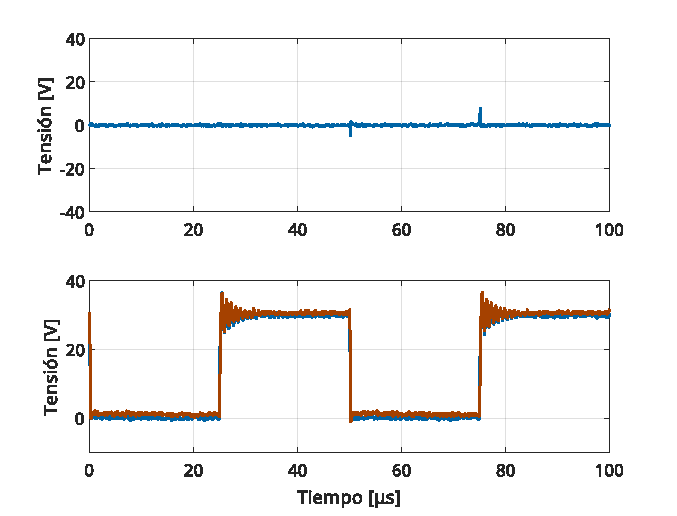
\includegraphics[width=\textwidth]{Imagenes/Sin Carga - Fase 0.pdf}
        \caption{Fase relativa de 0°.}
        \label{fig:ensayo_sincarga0}
    \end{subfigure}
    \hspace{0.5em}
    \begin{subfigure}{0.47\textwidth}
        \centering
        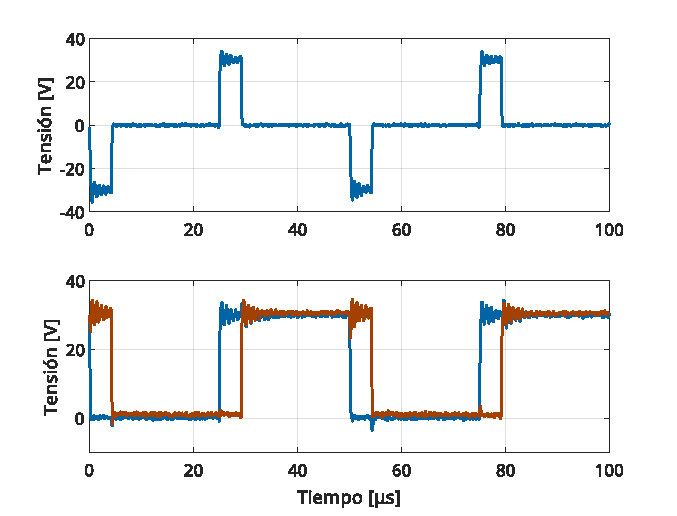
\includegraphics[width=\textwidth]{Imagenes/Sin Carga - Fase 30.pdf}
        \caption{Fase relativa de 30°.}
        \label{fig:ensayo_sincarga30}
    \end{subfigure}
    \hfill\vspace{1em}
    \begin{subfigure}{0.47\textwidth}
        \centering
        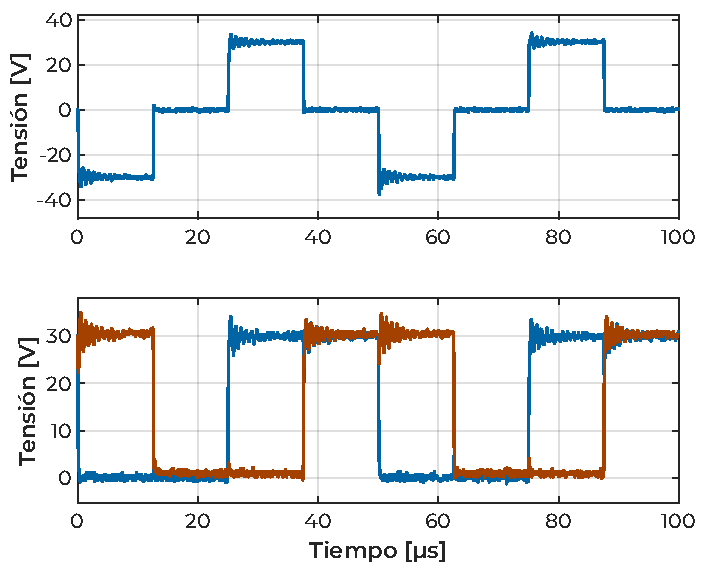
\includegraphics[width=\textwidth]{Imagenes/Sin Carga - Fase 90.pdf}
        \caption{Fase relativa de 90°.}
        \label{fig:ensayo_sincarga90}
    \end{subfigure}
    \hspace{0.5em}
    \begin{subfigure}{0.47\textwidth}
        \centering
        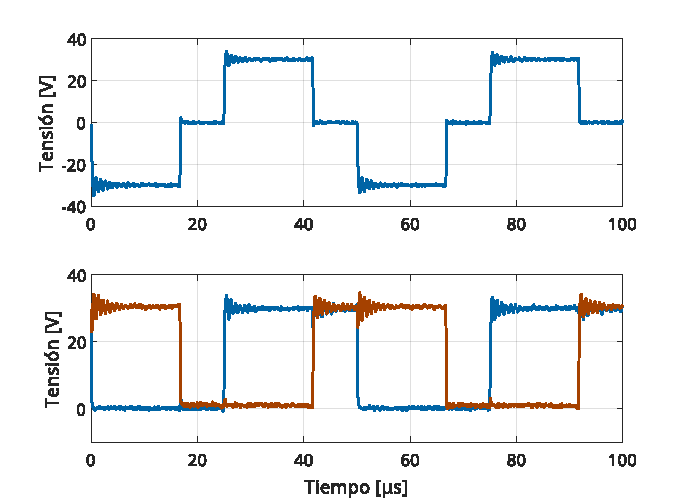
\includegraphics[width=\textwidth]{Imagenes/Sin Carga - Fase 120.pdf}
        \caption{Fase relativa de 120°.}
        \label{fig:ensayo_sincarga120}
    \end{subfigure}
    \caption{Resultados de la medición de tensión de bobinado primario $V_p$ y tensiones de medios puentes $V_p^+$ y $V_p^-$.}
    \label{fig:ensayo_sincarga}
\end{figure}

Se pueden observar en la figura \ref{fig:ensayo_sincarga} las señales de tensión de bobinado primario y de ambos medios puentes medidas con el osciloscopio durante la realización del ensayo. Las señales de tensión de los medios puentes consisten en ondas cuadradas de \SI[]{20}{\kilo\hertz} de frecuencia fundamental y ciclo de trabajo $D$ fijo de 50\%, mientras que como tensión del bobinado se toma la diferencia de ambas ondas cuadradas. Así, entonces, se produce la forma de tensión \quotes{escalonada} y bipolar, comúnmente llamada onda cuadrada modificada, que se ve en las figuras \ref{fig:ensayo_sincarga30}, \ref{fig:ensayo_sincarga90} y \ref{fig:ensayo_sincarga120}.\\

Este ensayo generó resultados satisfactorios, ya que las ondas cuadradas del medio puente y la onda cuadrada modificada del primario se pueden ver claramente, con flancos de subida y bajada bien definidos y tiempos de establecimiento casi imperceptibles frente al período de \SI[]{50}{\micro\second}. Esto nos indica que el circuito de excitación está funcionando correctamente, y es capaz de disparar rápida y efectivamente a los transistores.\\

Sin embargo, en la figura se pueden notar artefactos de \textit{ringing} en todos los flancos de subida de las señales: fenómenos transitorios con oscilaciones de alta frecuencia que se suelen presentar a la hora de conmutar una llave por la que circulan grandes corrientes (y en líneas generales para sistemas de banda limitada). Estas oscilaciones consumen energía que de otra manera hubiese llegado a la salida del convertidor, reduciendo la eficiencia energética total del sistema. Además, generan sobrepicos de tensión sobre las llaves que, en casos extremos, pueden llegar a dañarlas o destruirlas.\\

Se puede ver también como este efecto se transmite por acoplamiento e interferencia electromagnética: cuando una de las ondas cuadradas tiene un flanco de subida, se puede ver una oscilación similar inducida en la otra señal cuadrada. En cualquier caso, la presencia del ringing en el caso de este ensayo no es de mayor preocupación, ya que los sobrepicos de tensión que genera son baja magnitud, de alrededor de \SI[]{7}{\volt} por encima de los \SI{30}{\volt} finales de la onda cuadrada, o alrededor del 23\%.\\

Habiendo obtenido un resultado exitoso del primer ensayo, se puede pasar al ensayo con carga, dónde se va a poder observar y evaluar el funcionamiento del convertidor completo en condiciones de carga moderadas, incluyendo transformación y rectificación de la tensión del bobinado primario.\\